% Figure 6.34 -- the full forward model, end to end.
%
% Source recovered from ~/Projects/NBody/IMAGES/main_pipeline.tex and reflowed
% for print. The original was a SINGLE row: 987 x 205 pt, an aspect ratio of
% 4.8:1, so at \textwidth (about 359 pt) it printed barely an inch tall and its
% \footnotesize labels came out near 3 pt -- a third of the caption beside them,
% with "Paint spherical" running into the next panel.
%
% This version wraps the chain onto TWO rows and raises every type size, so the
% canvas is about 1.4:1 and the labels land near the caption's own size once
% scaled to \textwidth. Each phase box sits wholly within one row, so no \fit
% straddles the wrap.
%
% The two density-cube PNGs carried baked-in "X [Mpc/h]" and "Y [Mpc/h]" axis
% names that printed near 5.4 pt against a 9 pt caption and gave no scale, since
% they carried no tick values and no sentence referred to them. They have been
% erased from 01_initial_conditions.png and 02_final_density.png down to the
% transparent background, leaving the canvas size and so this layout untouched.
%
% Copied from the thesis (figures/chap6/pipeline.tex) for the jax-fli README, with the
% Rubin telescope replaced by Euclid (pipeline_images/telescope_euclid.png, rendered
% from slides/assets/PhD/1_intro/telescopes/telescope_euclid.svg with `rsvg-convert -w 1000`).
% pipeline_thesis.pdf is the thesis build, kept for reference.
%
% Build:
%   cd assets/pipeline && pdflatex -interaction=nonstopmode pipeline.tex
%   pdftocairo -svg pipeline.pdf ../PIPELINE.svg
\documentclass[border=12pt,tikz]{standalone}
\usepackage[T1]{fontenc}
\usepackage{helvet}
\renewcommand{\familydefault}{\sfdefault}
\usepackage{sfmath}
\usepackage{graphicx}
\usepackage{tikz}
\usepackage{xcolor}
\usepackage{amsmath,amssymb}

\usetikzlibrary{
  arrows.meta,
  calc,
  decorations.pathreplacing,
  positioning,
  shapes.geometric,
  fit,
  backgrounds,
}

% -- colours (light theme) --------------------------------------
\definecolor{fgdark}{HTML}{1F2328}
\definecolor{fgmuted}{HTML}{656D76}
\definecolor{arrowcolor}{HTML}{D97706}    % amber arrows
\definecolor{nodeoutline}{HTML}{D0D7DE}
\definecolor{nodefill}{HTML}{F6F8FA}

% phase box tints (high-alpha / very light)
\definecolor{priorfill}{HTML}{EAF2FB}
\definecolor{priorline}{HTML}{9EC5F0}
\definecolor{likefill}{HTML}{FBF1E4}
\definecolor{likeline}{HTML}{E8B876}
\definecolor{obsfill}{HTML}{EAF6EE}
\definecolor{obsline}{HTML}{95CBA6}

% -- styles ------------------------------------------------------
% Type sizes are set one to two steps above the original: the canvas is about
% 18 cm wide and prints at 12.6 cm, so a \large label lands near 9 pt on the
% page, matching the caption.
\tikzset{
  flow/.style={
    -{Stealth[length=9pt,width=7pt]},
    line width=2.2pt, arrowcolor,
  },
  busline/.style={line width=2.2pt, arrowcolor},
  flowlabel/.style={
    font=\LARGE\sffamily, text=fgmuted,
    fill=none, inner sep=3pt,             % transparent background
  },
  seclabel/.style={font=\huge\bfseries\sffamily},
  caplabel/.style={font=\LARGE\sffamily, text=fgdark, align=center},
  imnode/.style={inner sep=0pt, outer sep=0pt},
  paramcirc/.style={
    circle, draw=nodeoutline, fill=nodefill,
    line width=1.4pt, minimum size=20mm,  % fixed diameter -> both equal
    font=\LARGE\sffamily, text=fgdark, inner sep=0pt,
  },
  phasebox/.style={rounded corners=7pt, line width=1.3pt},
}

\begin{document}
\begin{tikzpicture}

% ===========================================================
%  ROW 1:  priors -> IC -> density -> shell
%  ROW 2:  lensing -> Euclid
%  The wrap sits on the Born step, which is also where the model
%  stops being a simulation and starts being an observable.
% ===========================================================
\def\rowone{3.6}
\def\rowtwo{-4.6}

% -- row 1 --
\node[paramcirc] (pomega) at (0,  \rowone+1.15) {$P(\boldsymbol\Omega)$};
\node[paramcirc] (pdelta) at (0,  \rowone-1.15) {$P(\delta_{\mathrm{ic}})$};

\node[imnode] (ic)     at ( 5.9, \rowone) {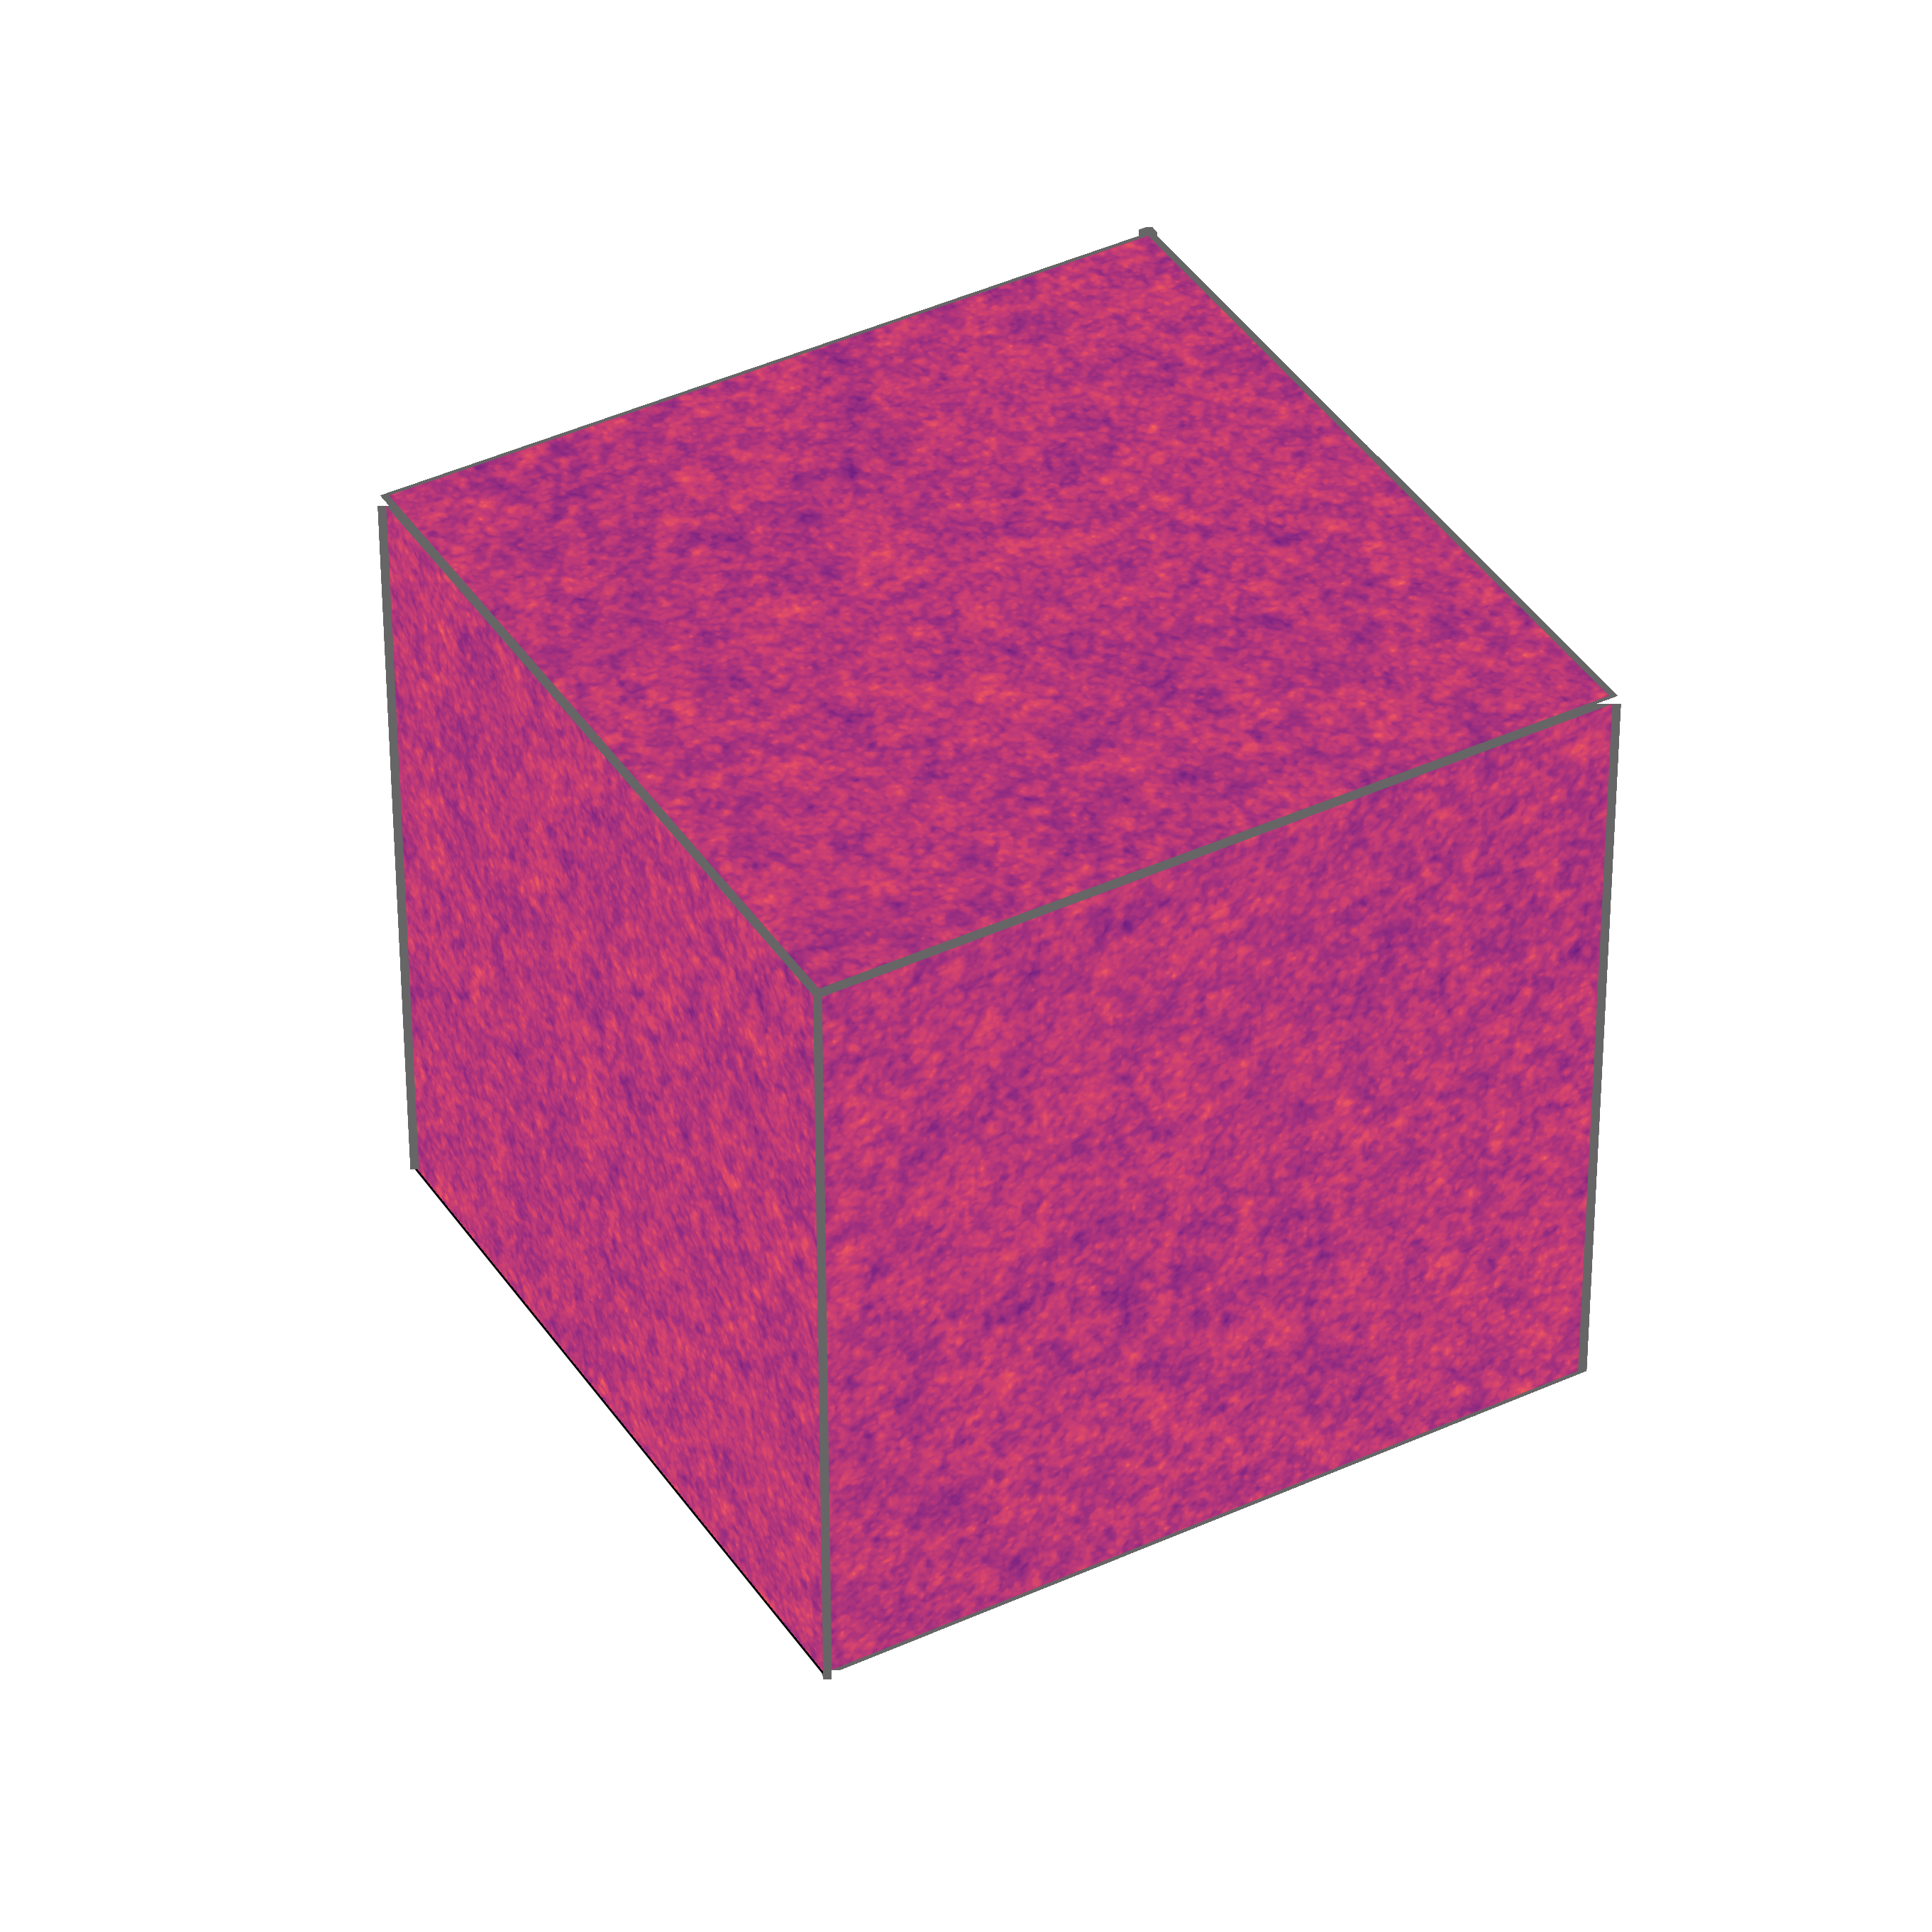
\includegraphics[height=3.6cm]{pipeline_images/01_initial_conditions.png}};
\node[imnode] (dens)   at (12.1, \rowone) {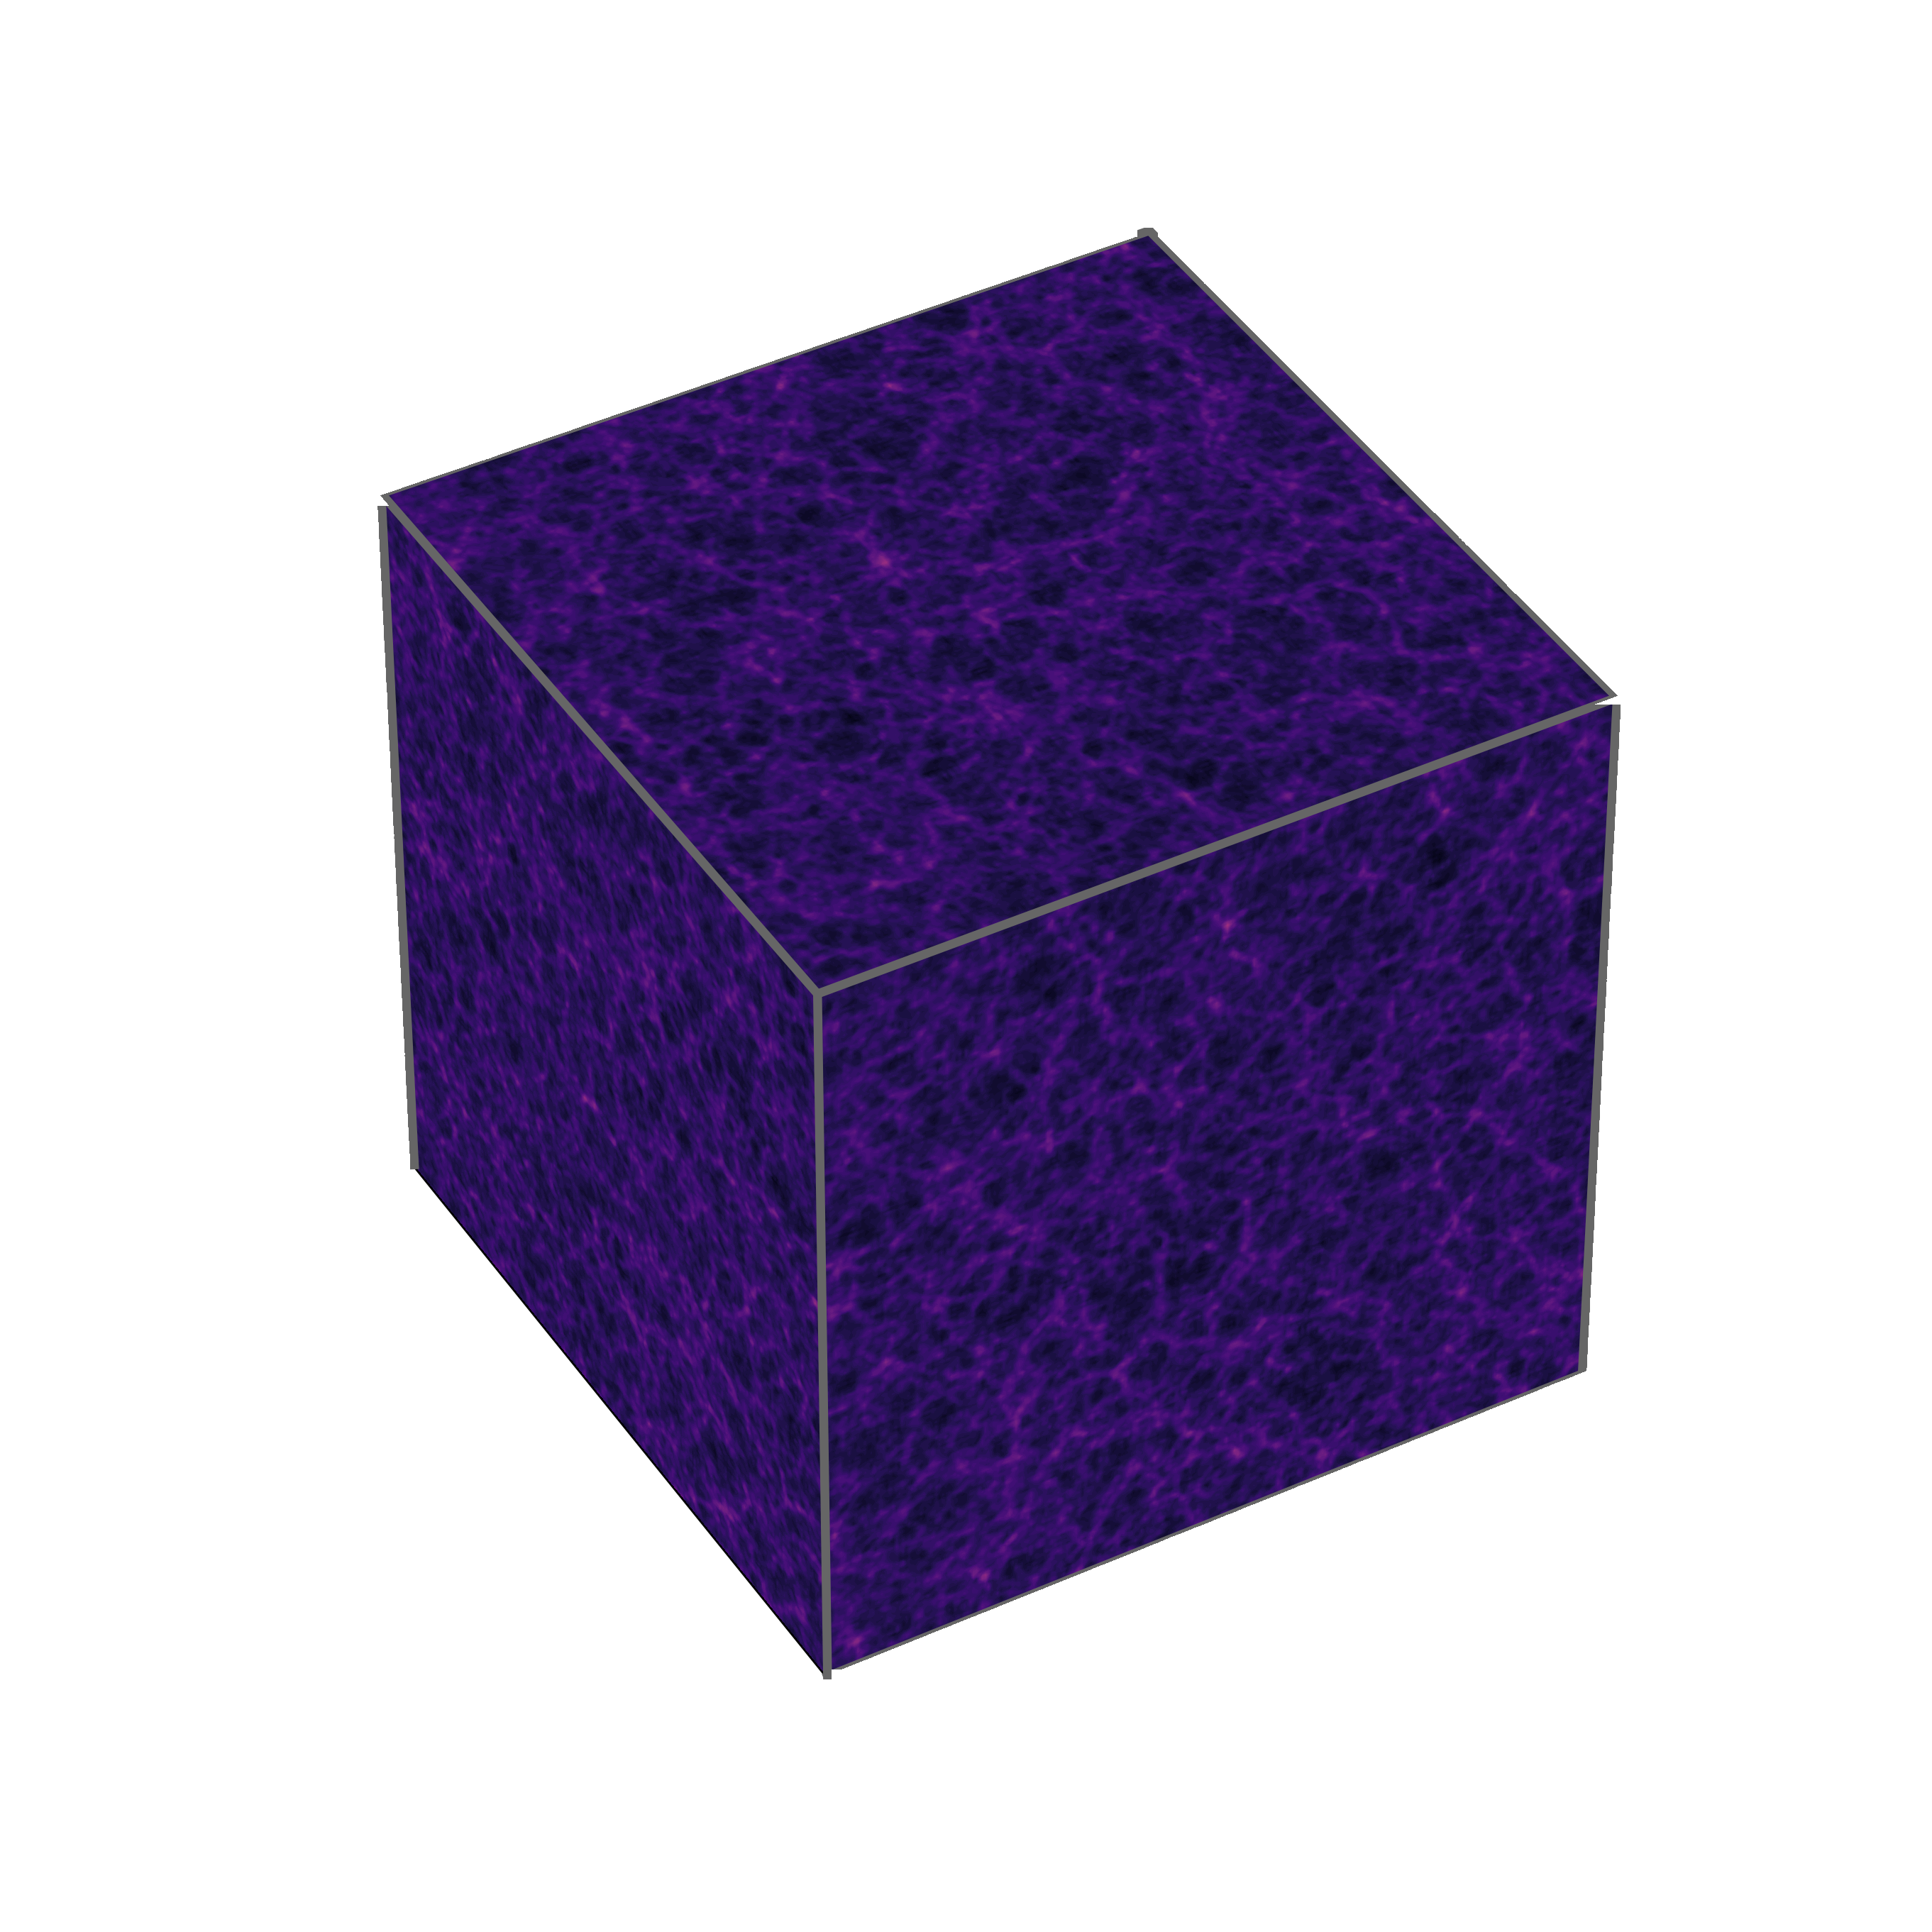
\includegraphics[height=3.6cm]{pipeline_images/02_final_density.png}};
\node[imnode] (sphere) at (18.3, \rowone) {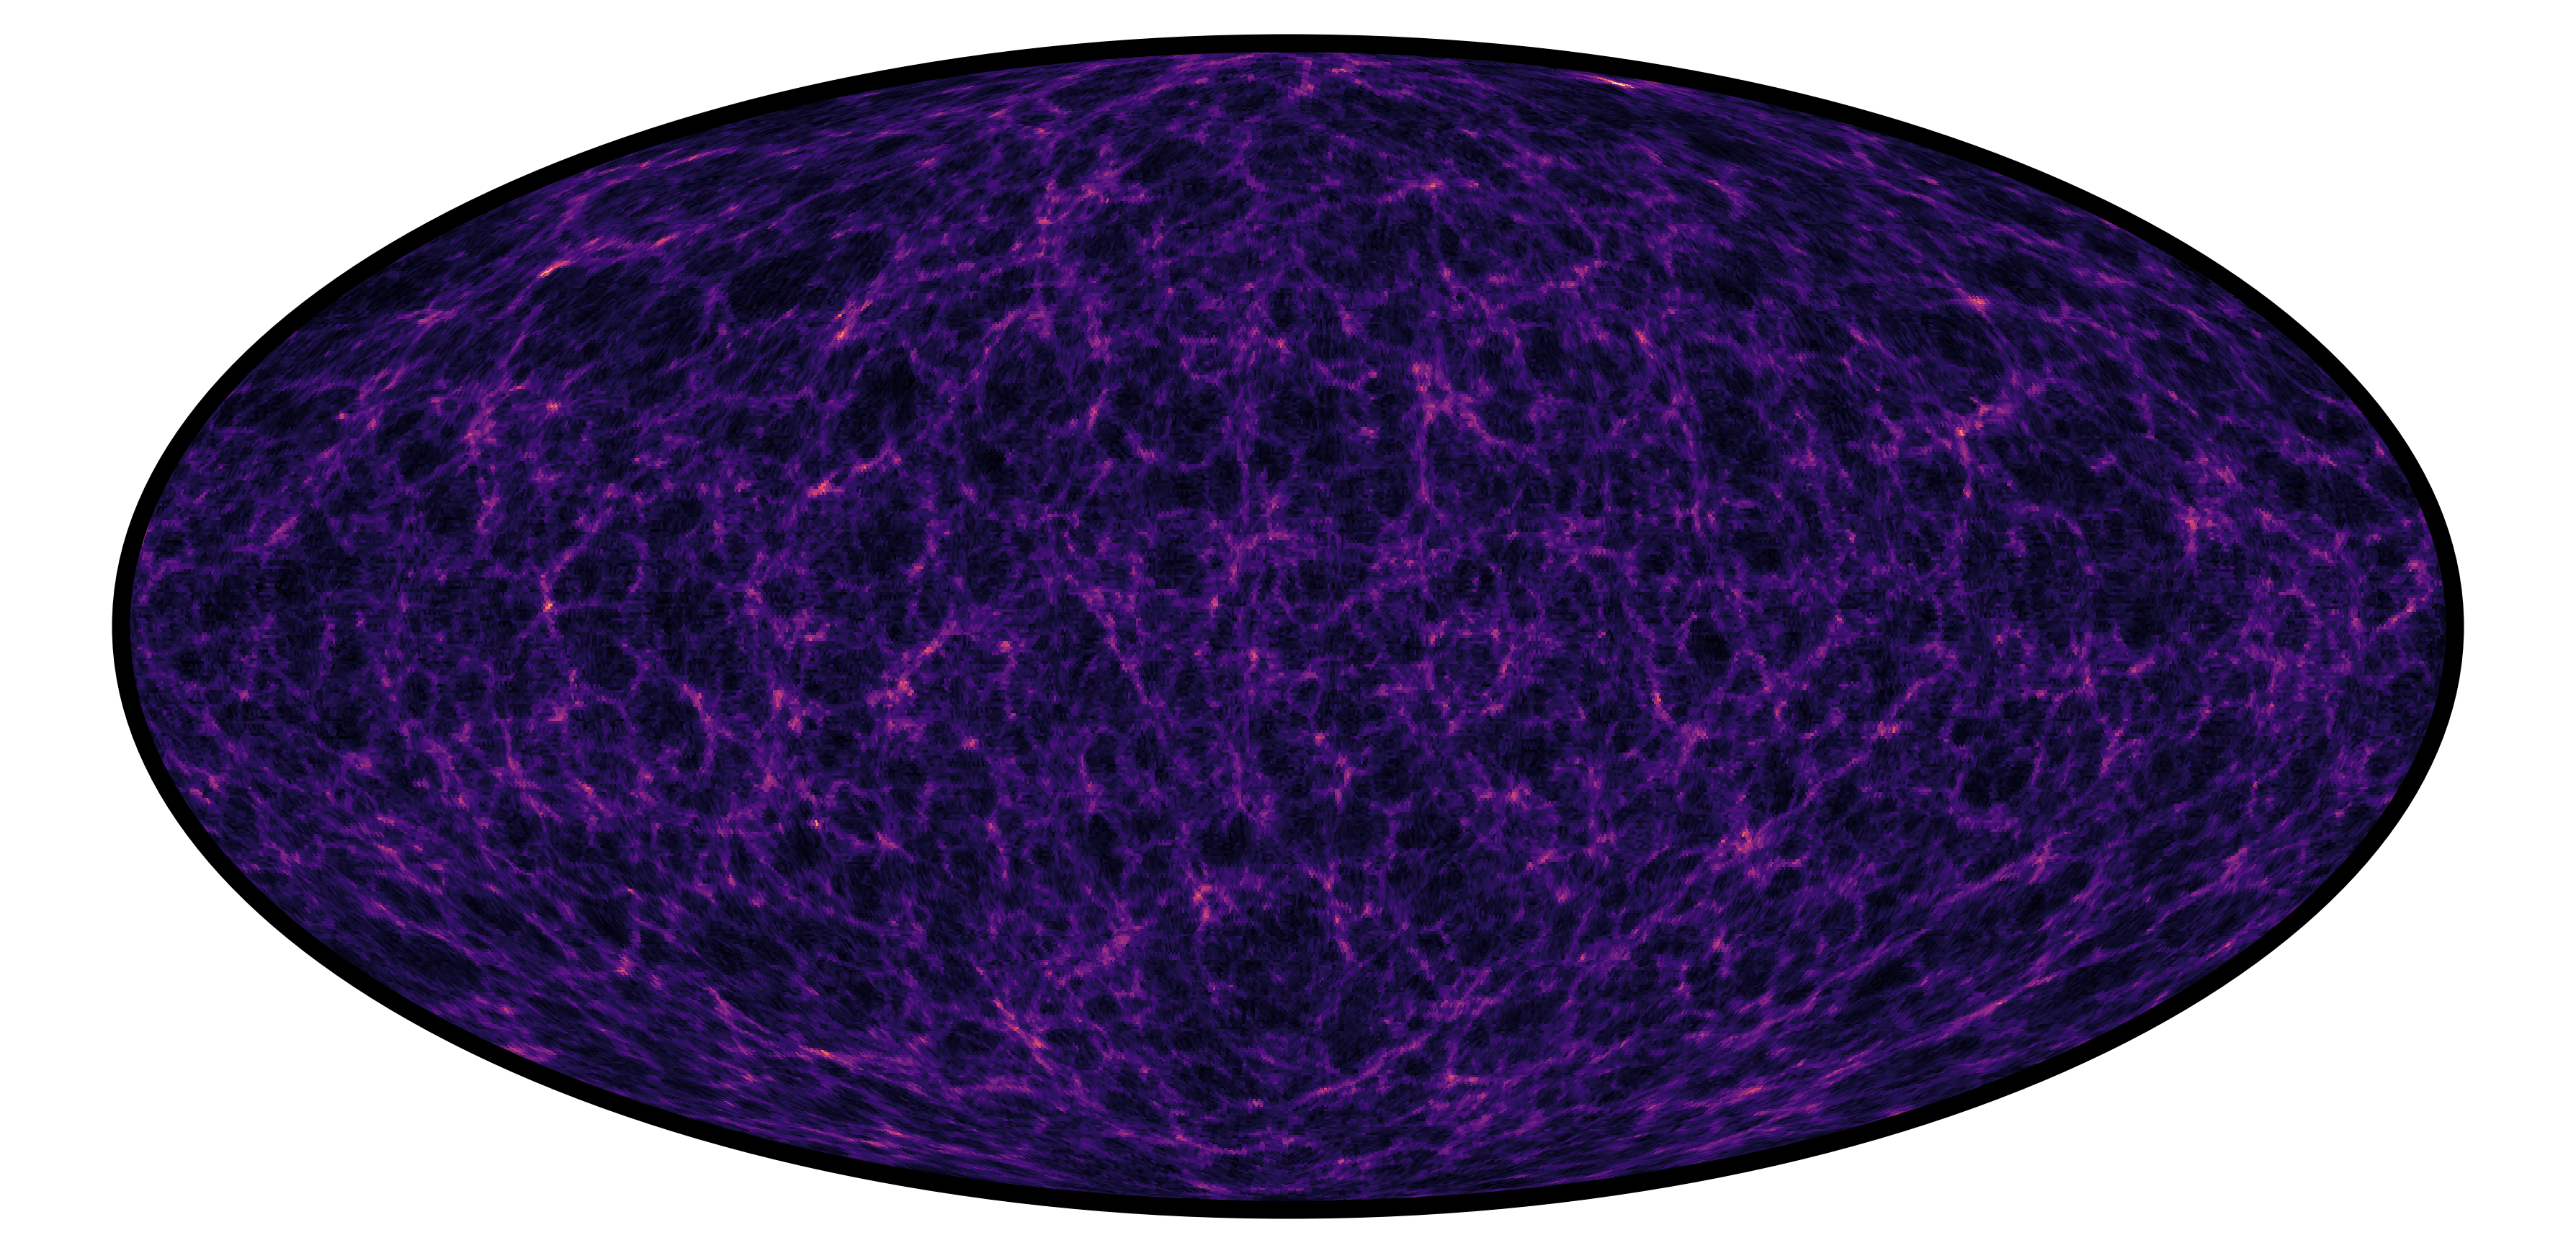
\includegraphics[height=2.9cm]{pipeline_images/03_spherical_projection.png}};

% -- row 2 --
\node[imnode] (lens)   at ( 6.4, \rowtwo) {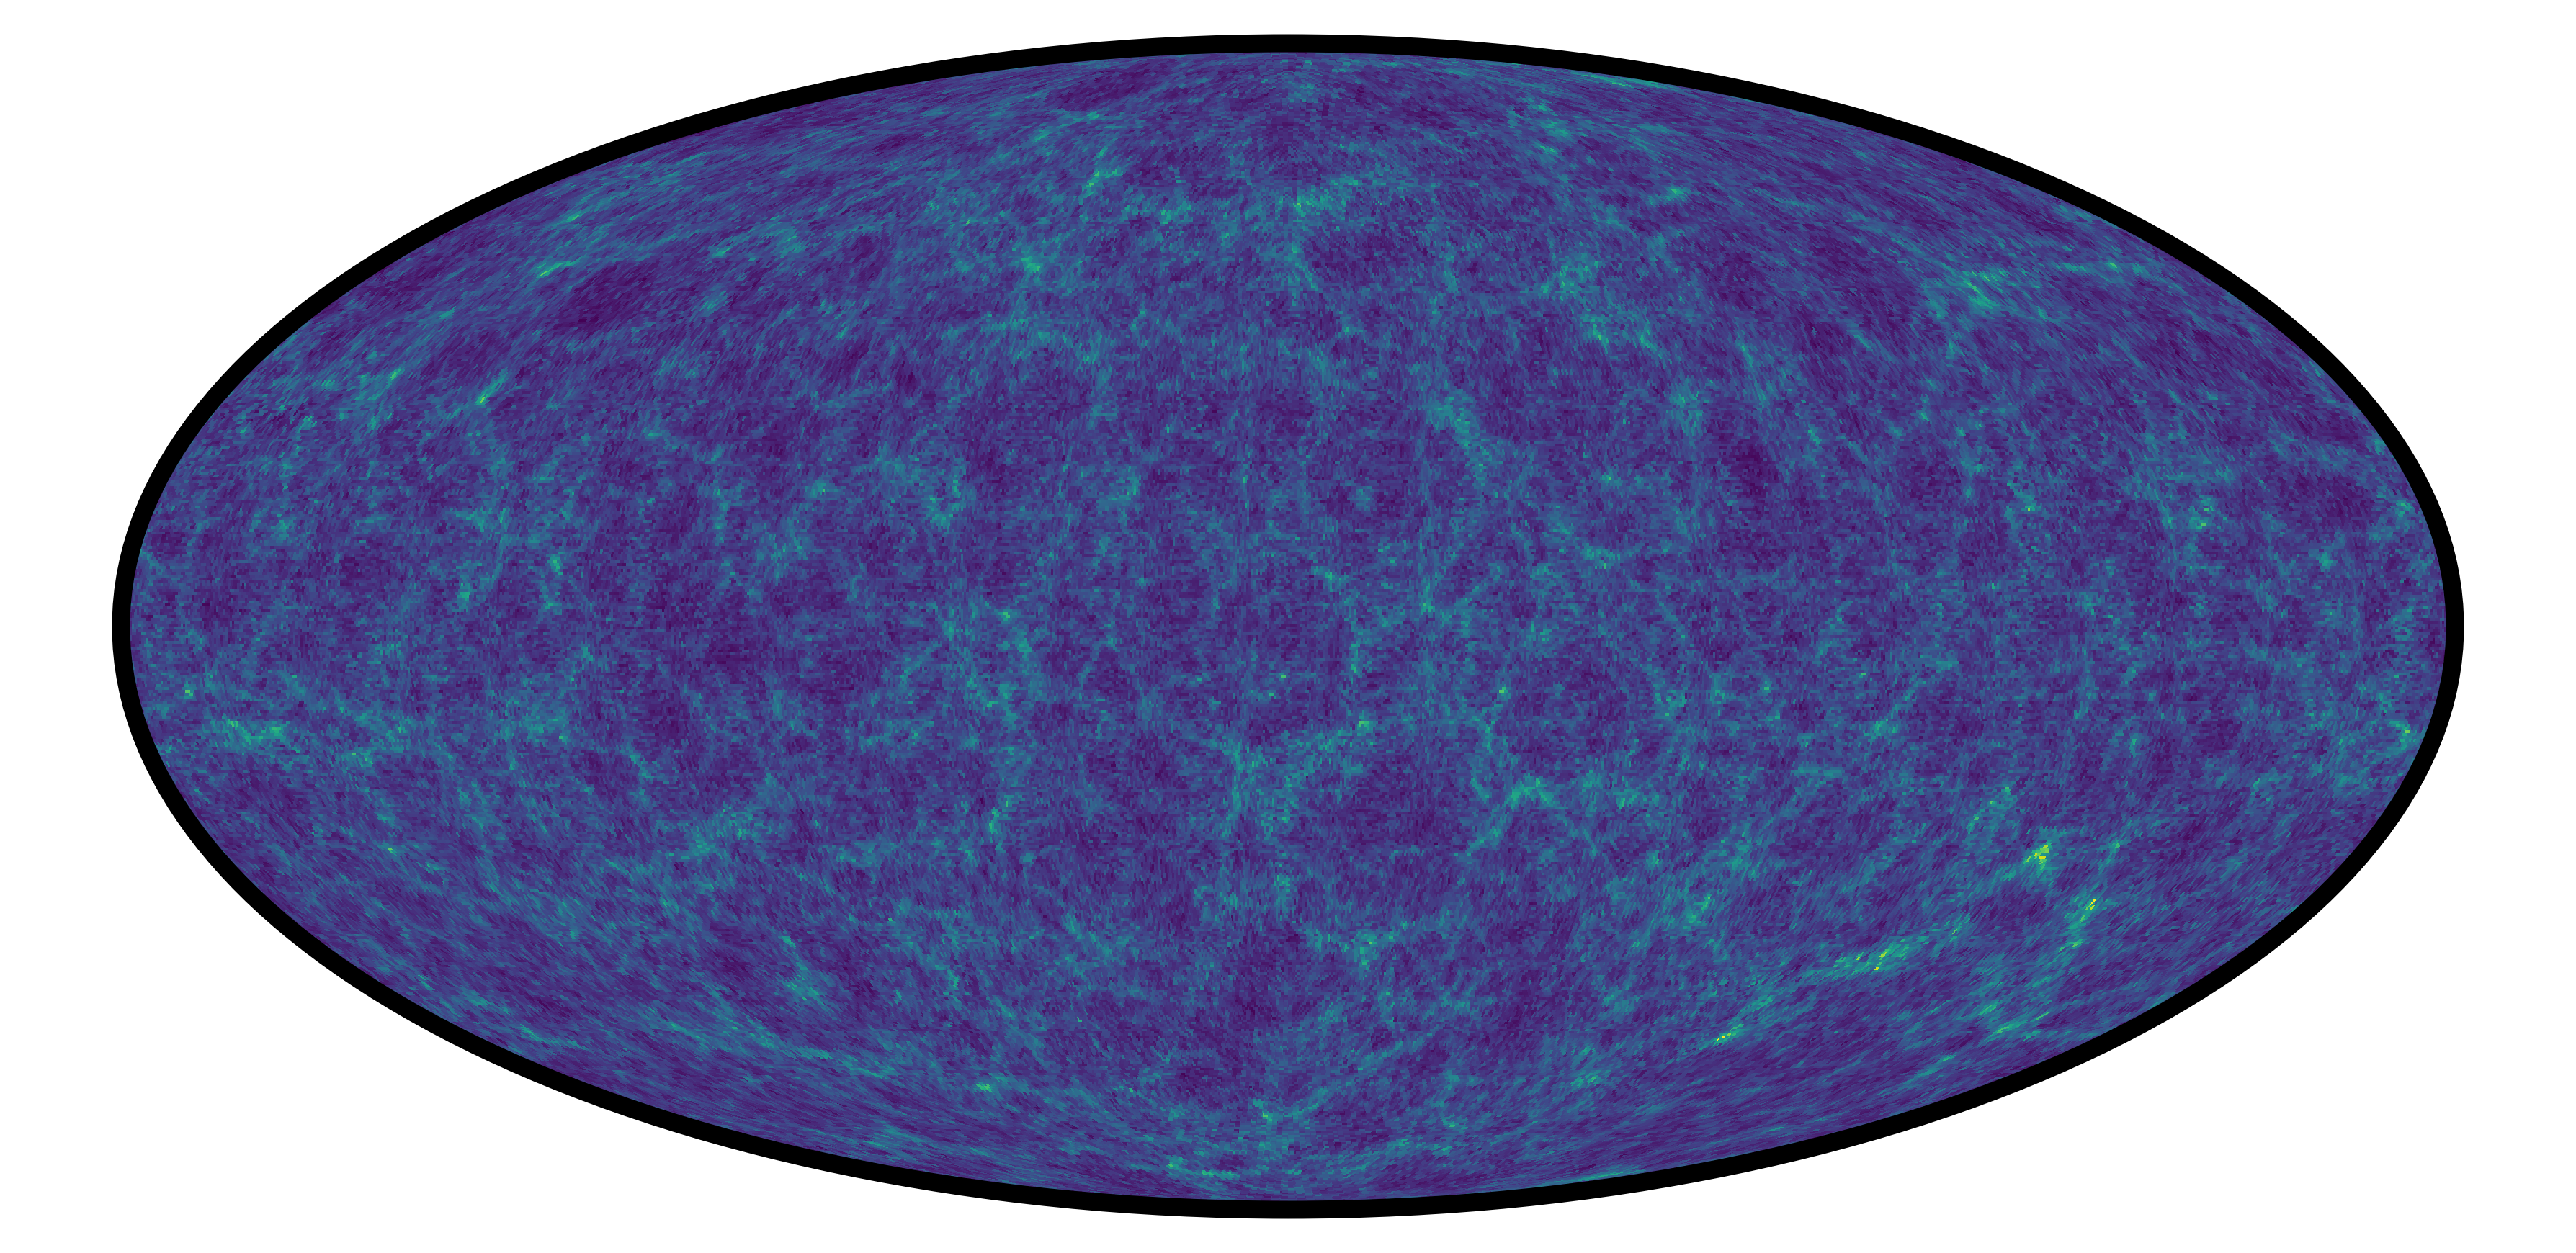
\includegraphics[height=2.9cm]{pipeline_images/04_lensing_map.png}};
\node[imnode] (euclid) at (14.2, \rowtwo) {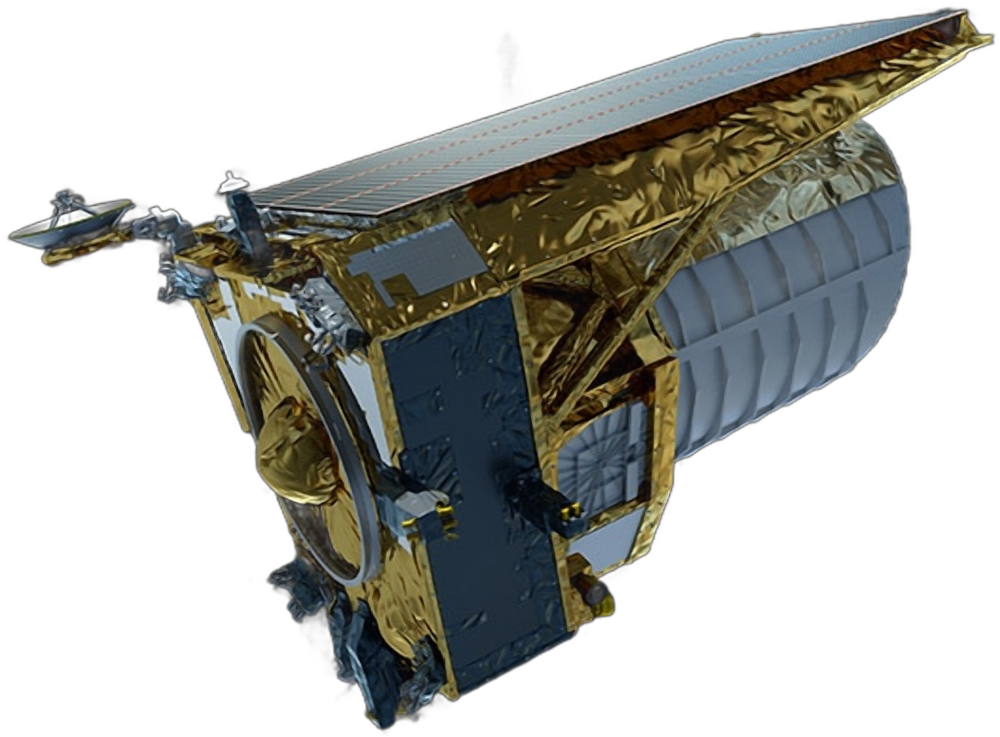
\includegraphics[height=3.4cm]{pipeline_images/telescope_euclid.png}};

% ===========================================================
%  CAPTIONS -- pinned per row
% ===========================================================
\node[caplabel, anchor=south] at ($(ic.center)    +(0,2.05)$) {Initial\\Conditions};
\node[caplabel, anchor=south] at ($(dens.center)  +(0,2.05)$) {Evolved\\Density Field};
\node[caplabel, anchor=south] at ($(sphere.center)+(0,2.05)$) {Light-Cone\\Shell};
\node[caplabel, anchor=south] at ($(lens.center)  +(0,1.75)$) {Lensing Map\\$\kappa\,/\,\gamma$};
\node[caplabel, anchor=south] at ($(euclid.center)+(0,1.75)$) {Euclid};

% ===========================================================
%  ARROWS
% ===========================================================
% Priors merge onto a common vertical bus, then a single arrow into IC.
% Both circles share a diameter, so both east anchors sit at the same x
% -> the two horizontal stubs are identical length and perfectly aligned.
\coordinate (merge) at ($(ic.west)+(-1.25,0)$);
\draw[busline] (pomega.east) -| (merge);
\draw[busline] (pdelta.east) -| (merge);
\draw[flow]    (merge) -- ([xshift=-4pt]ic.west);

\draw[flow] ([xshift=1pt]ic.east) -- ([xshift=-1pt]dens.west)
  node[flowlabel, midway, below=2.15cm] {PM $N$-body};

\draw[flow] ([xshift=1pt]dens.east) -- ([xshift=-4pt]sphere.west)
  node[flowlabel, midway, below=2.15cm] {Paint spherical};

% The wrap: out of the shell, down between the rows, back to the lensing map.
% Routed round the right so it never crosses a phase box.
\coordinate (wrapa) at ($(sphere.east)+(1.5,0)$);
\coordinate (wrapb) at ($(wrapa)+(0,-4.3)$);
\coordinate (wrapc) at ($(lens.west)+(-1.5,0)$);
\draw[busline] ([xshift=6pt]sphere.east) -- (wrapa);
\draw[busline] (wrapa) -- (wrapb);
\draw[busline] (wrapb) -| ($(wrapc)+(0,0)$)
  node[flowlabel, pos=0.5, above=4pt] {Born};
\draw[flow]    (wrapc) -- ([xshift=-6pt]lens.west);

\draw[flow] ([xshift=6pt]lens.east) -- ([xshift=-6pt]euclid.west)
  node[flowlabel, midway, below=1.95cm] {Observe};

% ===========================================================
%  PHASE BOXES  -- each fits wholly inside one row
% ===========================================================
\begin{scope}[on background layer]
  \node[phasebox, fill=priorfill, draw=priorline,
        fit=(pomega)(pdelta)(ic), inner xsep=13pt, minimum height=6.9cm] (priorbox) {};
  \node[phasebox, fill=likefill, draw=likeline,
        fit=(dens)(sphere), inner xsep=13pt, minimum height=6.9cm] (likebox) {};
  \node[phasebox, fill=obsfill, draw=obsline,
        fit=(lens)(euclid), inner xsep=13pt, minimum height=6.3cm] (obsbox) {};
\end{scope}

% phase labels -- centred above each box
\node[seclabel, text=priorline!60!fgdark, anchor=south] at (priorbox.north) {Prior};
\node[seclabel, text=likeline!60!fgdark,  anchor=south] at (likebox.north)  {Forward};
\node[seclabel, text=obsline!55!fgdark,   anchor=south] at (obsbox.north)   {Observable};

\end{tikzpicture}
\end{document}
